\chapter{Ejercicios y soluciones}

\section*{Enero 2023}
\addcontentsline{toc}{section}{Enero 2023} 
\setcounter{section}{1} % Configura manualmente el contador de secciones


\begin{ejercicio}
	La estrucutra de la figura está formada por átomos de Bi en los nodos de una \fcc, y átomos de Li en todos los huecos octaédricos de dicha \fcc \ de átomos de Bi. El lado de la sc es $a=6.74 \unit{\Angstrom}$. Responde a:
	\begin{enumerate}
		\item ¿Cuál es su forma estequiométrica?
		\item ¿Cuantas ramas de vibración y de qué tipo presenta esta estructura?¿Podrían estar degeneradas para algunas direcciones cristalográficas? En tal caso, explica por qué y pon algún ejemplo (indicando la dirección y las ramas que estarían degeneradas).
		\item Calcula la temperatura de Debye y el calor específico a 300K. Dato: velocidad del sonido en ese material es 1029 m/s. 
	\end{enumerate}
	\begin{center}
		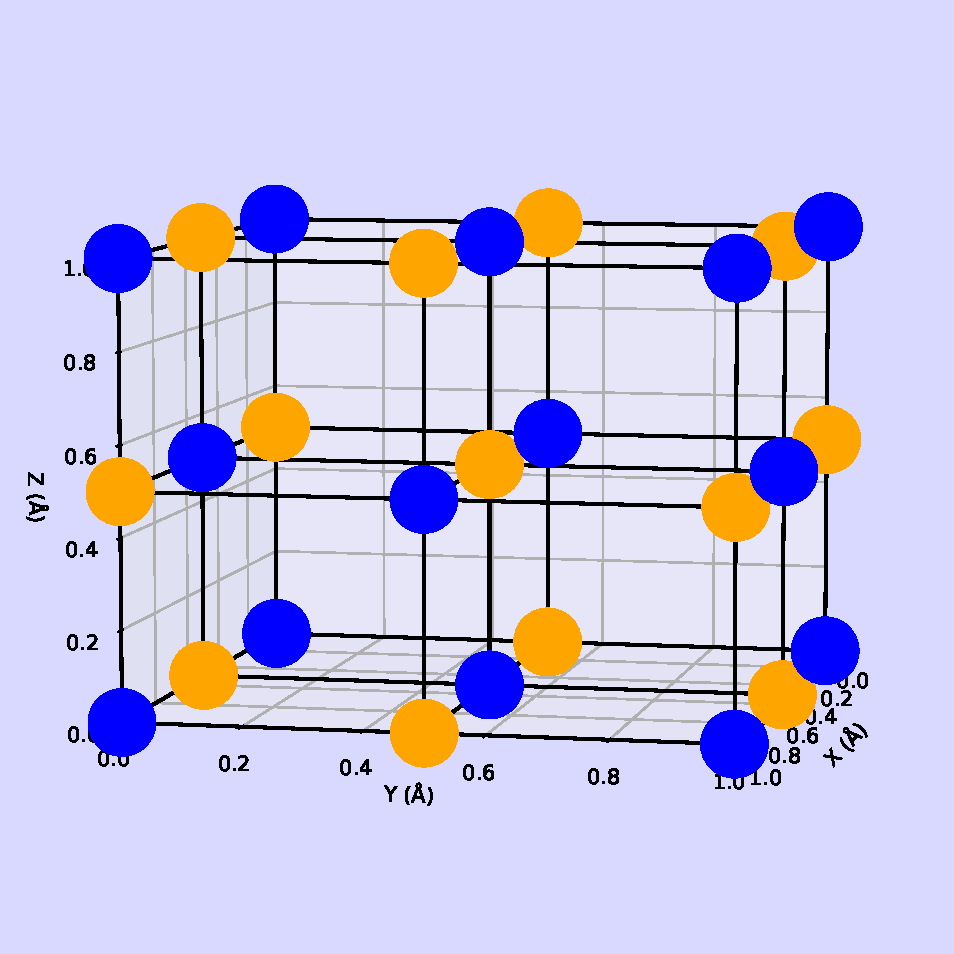
\includegraphics[scale=0.5]{Imagenes/2023-Enero-01.pdf}
	\end{center}
		
\end{ejercicio}	

\begin{ejercicio}
	Sea la red hexagonal simple de la figura ($a=3 \unit{\Angstrom},\ c=4 \unit{\Angstrom}$). 
	\begin{enumerate}
		\item Dibuja sobre la figura unos vectores base e indica las componentes.
		\item Calcula la red recíproca. ¿De qué tipo de red se trata?
		\item Una muestra de polvo con esta estructura se ilumina con RX (rayos X) de longitud de onda $\lambda = 5 \unit{\Angstrom}$. Determina los picos de difracción de menor y mayor ángulo.
		\item Calcula la relación de dispersión electrónica en el marco de la aproximación de electrones fuertemente ligados, utilizando solo orbitales $s$ y teniendo en cuenta hasta segundos vecinos. Calcula las masas efectivas electrónicas $m_x^*,m_y^*$ y $m_z^*$ cerca del fondo de la banda. Datos: $\gamma_1 = 0.4 \ \unit{eV}, \ \gamma_2 = 0.2 \ \unit{eV}$.
		\item Cada átomo aporta un electrón a la conducción, y entre la PZB y la SZB hay un gap de energía despreciable. Indica si el metal es aislante, metal, semimetal o semicondcutor, y que bandas contribuirían a la conducción eléctrica. Justifica las respuestas.
	\end{enumerate}
\end{ejercicio}	


\begin{ejercicio}
	Un semiconductor extraído de una computadora tiene como parámetros $\varepsilon_g = 1$ eV, $m_e^* = m_h^* = m_e$. Está dopado con una concentración de aceptores de $N_A = 10^{16} \unit{cm}^{-3}$. Calcular la concentración de electrones y huecos a 300 K. 
\end{ejercicio}	


\begin{solucion}
	\begin{enumerate}
		\item La fórmula estequiométrica es evidente: Li$_3$Bi.
		\item Como sabemos las ramas de vibración dependen de dos factores: la dimensión de la estructura $D$ y el número de átomos dentro de la base atómica $z$. La ecuación es:
		
		\begin{equation}
			\text{Acústicas:} \quad D  \tquad
			\text{Ópticas:} \quad D(z-1)
		\end{equation}
		En nuestro caso $D=3$ y $z=4$. Entonces tenemos 3 ramas acústicas y 9 ramas ópticas, obteniendo los 12 modos normales esperados. 
		
		
		\item Como sabemos la temperatura de Debye viene dada por la ecuación
		\begin{equation*}
			\theta_D= \frac{\hbar \omega_D}{k_B}
		\end{equation*}
		Mientras que la velocidad del sonido $c$ nos permite relacionar $\omega$ Y $k$ tal que $\omega = c k$. Y, como sabemos que $k_D$ viene dada por
		
		\begin{equation*}
			k_D^3 = 6 \pi^2 n
		\end{equation*}
		siendo $n=zN/V$ la densidad numérica de átomos. Entonces podemos obtener $\theta_D$ a partir de los datos dados, ya que $z=4$ y $N/V$ es exactamente igual al número de puntos de red por celda, tal que $N/V=4/a^3$. Entonces:
		
		\begin{equation}
			\theta_D = \frac{\hbar}{k_B} c \sqrt[3]{6\pi^2 n} \longrightarrow \theta_D = 
		\end{equation}
		La capacidad calorífica a la temperatura $T$ viene dada por la ecuación a temperaturas tal que
		
		\begin{equation}
			C_V = 
		\end{equation} 
		de lo que se deduce 
		
		\begin{equation}
			C_V = 
		\end{equation}
		
	\end{enumerate}
	
\end{solucion}	

\section*{Enero 2021}
\addcontentsline{toc}{section}{Enero 2021} 
\setcounter{section}{2} % Configura manualmente el contador de secciones

\section*{Enero 2020}
\addcontentsline{toc}{section}{Enero 2020} 
\setcounter{section}{3} % Configura manualmente el contador de secciones

\section*{Julio 2019}
\addcontentsline{toc}{section}{Julio 2019} 
\setcounter{section}{4} % Configura manualmente el contador de secciones


\section*{Enero 2019}
\addcontentsline{toc}{section}{Enero 2019} 
\setcounter{section}{5} % Configura manualmente el contador de secciones


